\documentclass[journal]{IEEEtran}

\ifCLASSINFOpdf
\else
   \usepackage [dvips]{graphicx}
\fi
\usepackage{url}

\hyphenation{op-tical net-works semi-conduc-tor}
% \newcommand{\blue}[1]{\textcolor{blue}{#1}}
\usepackage{graphicx}
\usepackage[caption=false,font=footnotesize]{subfig}
\usepackage{amssymb}
\usepackage{amsmath}

\begin{document}

\title{FSC-Net: Integrating Fast Fourier Convolutions and Progressive Learning for Speech Bandwidth Extension}
\author{Xinan Chen, Xiaobin Rong, Qinwen Hu, Kai Chen, \IEEEmembership{Member, IEEE}, and Jing Lu, \IEEEmembership{Senior Member, IEEE}
\thanks{Manuscript received xxxxxxx xx, 202X; revised xxxxxxx xx, 202X; accepted xxxxxxx xx, 202X. Date of publication xxx xx, 202X; date of current version xxx xx, 202X. This work was supported by the National Natural Science Foundation of China under Grant 12274221. The associate editor coordinating the review of this manuscript and approving it for publication was xxx. (Corresponding author: Kai Chen.)}
\thanks{Xinan Chen, Xiaobin Rong, Qinwen Hu and Jing Lu are with the Key Laboratory of Modern Acoustics, Nanjing University, Nanjing 210008, China, and also with NJU-Horizon Intelligent Audio Lab, Horizon Robotics, Beijing 100094, China (e-mails: \{xinan.chen, xiaobin.rong, qinwen.hu\}@smail.nju.edu.cn; lujing@nju.edu.cn).}
\thanks{Kai Chen is with the Key Laboratory of Modern Acoustics, Nanjing University, Nanjing 210008, China (e-mail: chenkai@nju.edu.cn).}
\thanks{The source code will be released upon acceptance of the paper. Demo: \protect\url{https://xinan-chen.github.io/FSC-Net-demo}.}}

\markboth{IEEE Signal Processing Letters,~Vol.~XX, No.~XX,~202X}
{Chen \MakeLowercase{\textit{et al.}}: FSC-Net: Integrating Fast Fourier Convolutions and Progressive Learning}
\maketitle

\begin{abstract}
Speech bandwidth extension (BWE) aims to reconstruct high-fidelity wideband audio from narrowband inputs. While recent approaches have made significant progress, they often struggle to reconstruct realistic high-frequency phase and harmonic structures, leading to perceptual artifacts. In this paper, we propose \textbf{FSC-Net} (Full-Spectrum Context Network), a parameter-efficient architecture designed to explicitly model cross-band harmonic dependencies. By integrating Fast Fourier Convolutions (FFCs) into a complex spectral mapping framework, FSC-Net expands its receptive field to the entire spectrum, capturing long-range frequency interactions effectively. To address the ill-posed nature of high-frequency generation, our novel frequency-progressive learning curriculum guides the network to reconstruct spectral details from coarse to fine. Experimental results on the VCTK and unseen EARS datasets demonstrate that FSC-Net delivers consistently strong reconstruction quality and generalization, particularly in the challenging VCTK 4~kHz-to-48~kHz task. Compared to scaled-up baselines, our model attains leading LSD and PESQ scores while maintaining a highly compact parameter footprint (1.54~M).
\end{abstract}


\begin{IEEEkeywords}
speech bandwidth extension, generative adversarial network, progressive learning, audio super-resolution
\end{IEEEkeywords}


\IEEEpeerreviewmaketitle



\section{Introduction}

Speech bandwidth extension (BWE) and audio super-resolution are fundamentally equivalent problems, both aiming to recover missing high-frequency spectral components. In practical speech communication systems, bandwidth limitations often degrade audio quality by truncating high-frequency components. BWE addresses this by reconstructing missing high-frequency content from narrowband signals \cite{iser2008bandwidth}. Early approaches relied on signal processing techniques including source-filter models \cite{makhoul1979high}, Line Spectral Frequencies (LSF) \cite{chennoukh2001speech}, codebook mapping \cite{carl1994bandwidth,unno2005robust}, and statistical methods using GMMs/HMMs \cite{jax2003artificial,park2000narrowband}, though these often produced over-smoothed spectral parameters \cite{ling2015deep}.

Recent deep learning methods fall into two categories: waveform-based approaches that directly map narrowband to wideband waveforms \cite{kuleshov2017audio,li2021real,kim2019bandwidth,su2021bandwidth,han2022nu}, and spectrum-based methods that predict high-frequency amplitudes while estimating phase through replication \cite{li2015deep,abel2018simple} or vocoders \cite{botinhao2006frequency}. Alternative approaches attempt phase recovery through STFT \cite{baenet,AP-BWE} or MDCT spectra \cite{shuai2023mdctgan}, but phase reconstruction remains challenging. 


For instance, AERO \cite{aero} incurs high computational costs and often produces metallic artifacts in the reconstructed high frequencies.
Similarly, AP-BWE \cite{AP-BWE} suffers from parameter explosion ($\sim$30~M) and heavy memory footprints due to stacked FC layers. Conversely, BAE-Net \cite{baenet} achieves efficiency via compressed FCs but lacks the capacity and global context to capture complex spectral dependencies. Even when scaled up with more parameters, such architectures often hit a performance bottleneck due to their limited receptive fields and lack of global context modeling. Recently, SFNet \cite{dai2025sfnet} introduced a highly efficient neural source-filter framework by integrating traditional digital signal processing (DSP) modules. However, its reliance on explicit pitch tracking can be fragile in extremely band-limited scenarios (e.g., 4~kHz).

These limitations motivate our improved approach. Inspired by advances in image restoration \cite{lama}, we propose FSC-Net (Full-Spectrum Context Network), which integrates Fast Fourier Convolutions (FFCs) into the efficient TF-GridNet backbone. Unlike the heavy FC layers in AP-BWE or the compressed ones in BAE-Net, our FFC module captures global spectral dependencies with minimal parameter overhead. 
\begin{figure*}[t]
\centerline{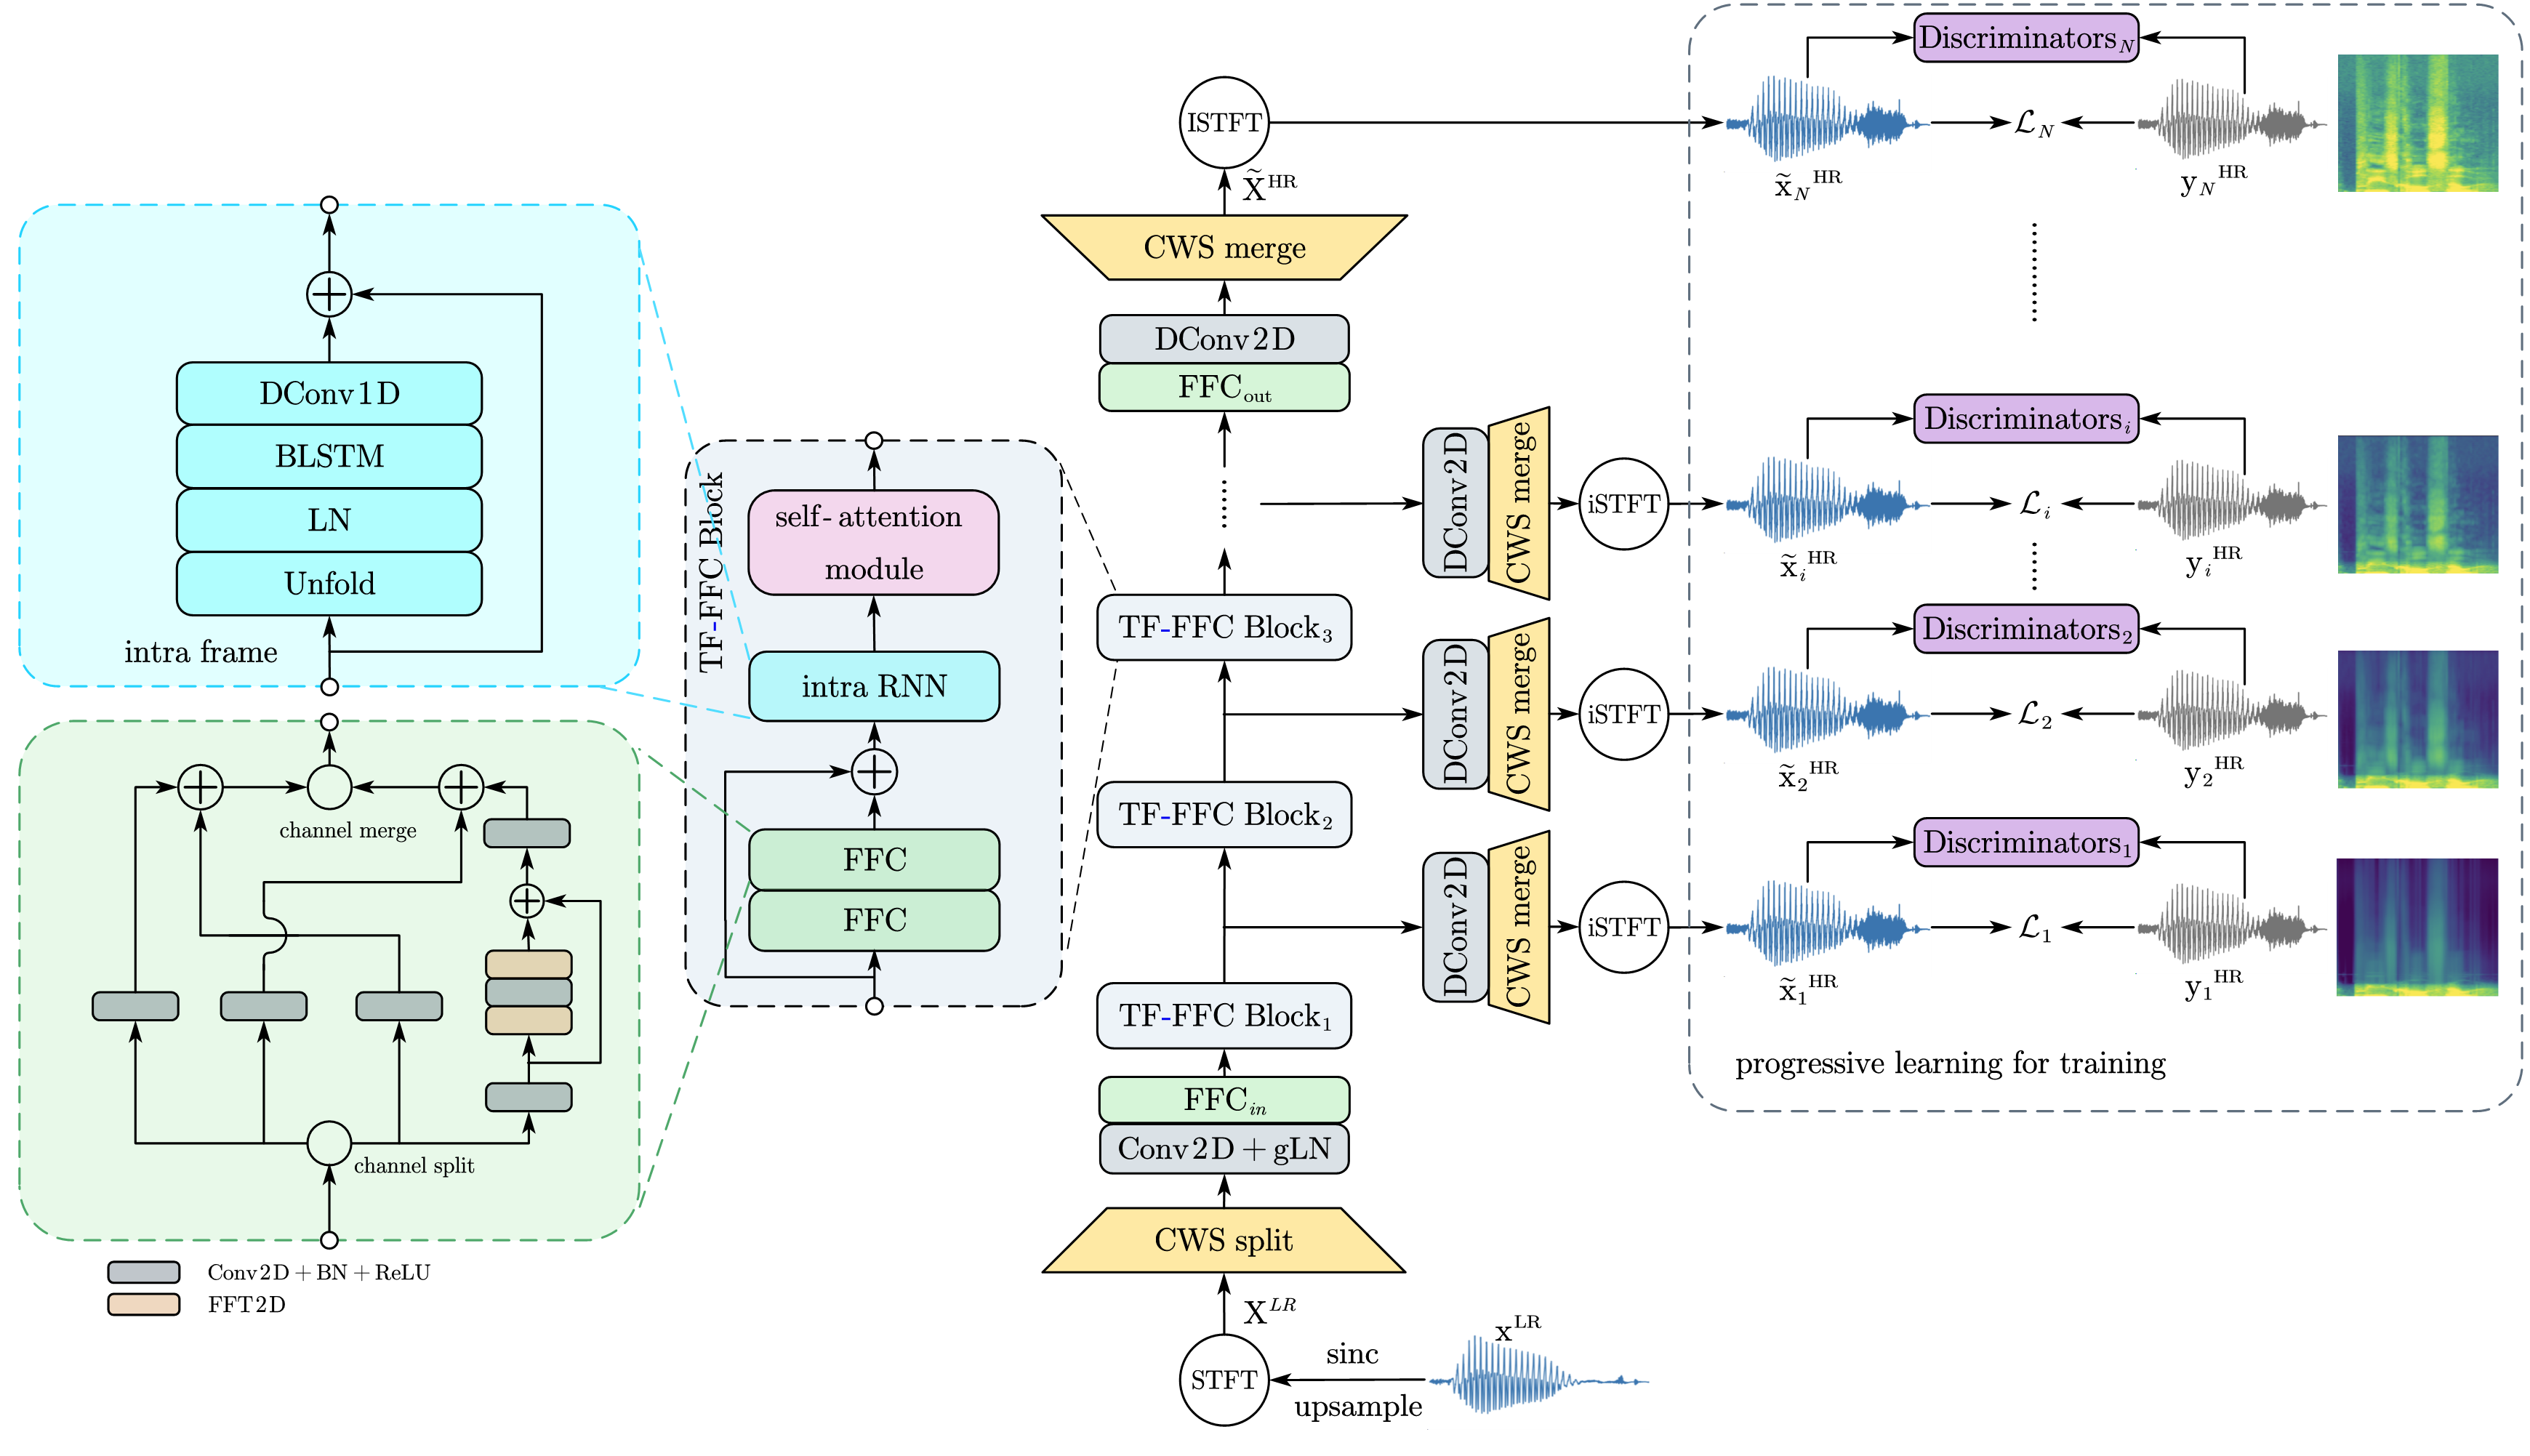
\includegraphics[width=\textwidth]{pic/FSCNet_struc.png}}
\vspace{-0.1cm}
\caption{The general architecture of FSC-Net and the framework for progressive learning. The model consists of $N$ TF-FFC Blocks, where $\hat{X}_i$ denotes the output of the $i$-th block. The $\text{FFC}_{in}$ and $\text{FFC}_{out}$ modules are consistent with the FFC module. Note that all intermediate outputs will not be used during model inference.
}
\label{main}
\vspace{-0.4cm}
\end{figure*}

Beyond architectural augmentation, we further introduce a novel frequency-progressive learning paradigm. Unlike existing SNR/SIR-progressive strategies that are specially designed for noise suppression \cite{hou2024snr, gao2016snr}, our approach fundamentally differs in the construction of intermediate targets: they are generated via a novel sliding-window averaging scheme applied exclusively to the high-resolution target spectrograms. Rather than directly targeting high-resolution reconstruction—which frequently yields artificial harmonics or spectral oversmoothing \cite{aero, jang2021univnet}—this coarse-to-fine design establishes a structured, multi-resolution reconstruction pathway. It stabilizes the recovery process by guiding the network to learn the global spectral envelope before refining fine-grained details. By integrating FSC-Net with this frequency-progressive curriculum, the model achieves superior preservation of phase coherence and harmonic structure, particularly in challenging extreme bandwidth extension scenarios (e.g., 4~kHz~$\to$~48~kHz).


\section{Methodology}

\subsection{Problem Formulation}
The goal of BWE is to estimate a high-resolution wideband waveform $\mathbf{y}^{\mathrm{HR}} \in \mathbb{R}^{T_{\mathrm{wb}}}$ from a given narrowband input waveform $\mathbf{x}^{\mathrm{LR}} \in \mathbb{R}^{T_{\mathrm{nb}}}$.  Given $\mathbf{x}^{\mathrm{LR}}$, we first obtain its complex spectrogram $X^{\mathrm{LR}} \in \mathbb{C}^{T \times F_{\mathrm{nb}}}$ via the Short-Time Fourier Transform (STFT).
The proposed FSC-Net acts as a complex spectral mapper $\mathcal{G}_\theta$, which takes $X^{\mathrm{LR}}$ (after upsampling to the target wideband rate) as input and predicts the full-band complex spectrogram $\hat{X}^{\mathrm{HR}} \in \mathbb{C}^{T \times F_{\mathrm{wb}}}$:
\begin{equation}
    \hat{X}^{\mathrm{HR}} = \mathcal{G}_\theta(\text{Pad}(X^{\mathrm{LR}})).
\end{equation}
The predicted wideband spectrogram is then transformed back to the time domain to obtain the predicted waveform $\hat{\mathbf{x}}^{\mathrm{HR}} = \text{iSTFT}(\hat{X}^{\mathrm{HR}})$, as illustrated in Fig.~\ref{main}.

\subsection{FSC-Net Architecture}
Our proposed model is built upon the TF-GridNet \cite{tfgridnet}, a state-of-the-art time-frequency domain model originally designed for speech separation. We adapt and enhance this architecture for the BWE task by introducing the following two key components.

\subsubsection{Channel-wise Subband (CWS) Processing}
 Given an input complex spectrogram $X \in \mathbb{C}^{T \times F}$, we partition the frequency dimension $F$ into $B$ subbands. These subbands are then stacked along the channel dimension, transforming the input into a tensor $X_{\mathrm{cws}} \in \mathbb{C}^{B \times T \times (F/B)}$. This CWS operation \cite{rong2025ts} allows the model to capture inter-subband dependencies through channel interactions while reducing the computational burden on the frequency axis. In our implementation, we set $B=3$.

\subsubsection{Fast Fourier Convolution (FFC) Integration}
To expand the receptive field for recovering missing high-frequency components correlated with low-frequency content, we replace TF-GridNet's time-domain inter-RNN with FFC modules \cite{lama}, retaining the intra-RNN. 
The FFC splits the input feature map into two branches: a local branch using standard convolutions and a global branch using spectral transforms. The global branch applies Real FFT to the feature map, performs convolutions in the frequency domain, and then applies Inverse Real FFT. Formally, for an input feature map $X$ the FFC output $Y$ is defined as:
\begin{equation}
    Y = \text{Conv2D}_{\mathrm{local}}(X) + \text{IFFT2D}(\text{Conv2D}_{\mathrm{global}}(\text{FFT2D}(X))).
\end{equation}
This mechanism provides the model with a global receptive field covering the entire spectrum, effectively bridging the ``spectral gap'' in BWE tasks.

\subsection{Progressive Learning Strategy}


Directly hallucinating high-frequency details in a single step often causes metallic artifacts \cite{aero}. To address this, we propose a coarse-to-fine frequency-progressive learning strategy (Fig.~\ref{main}), supervising each of the $N$ TF-FFC Blocks with a progressive target $|Y_{i}|$. Rather than smoothing the target directly, we apply sliding-window averaging to the magnitude residual $R(t, f) = |Y^{\mathrm{HR}}(t, f)| - |X^{\mathrm{HR}}(t, f)|$ between the ground-truth and input spectrograms. For the $i$-th stage, the target is computed as:
\begin{equation}
    |Y_{i}(t, f)| = |X^{\mathrm{HR}}(t, f)| + \frac{1}{W_i} \sum_{\delta=-\left\lfloor W_i/2 \right\rfloor}^{\left\lfloor W_i/2 \right\rfloor} R(t, f+\delta),
\end{equation}
where $W_i \in \{257, 65, 17, 5, 1\}$ is a decreasing sequence of window sizes, with zero-padding at frequency boundaries. Early blocks use larger $W_i$ to learn the global spectral envelope of missing components, while deeper blocks use smaller $W_i$ to refine fine harmonic structures. Ultimately, $W_N = 1$ strictly recovers the exact ground truth ($|Y_{N}| = |Y^{\mathrm{HR}}|$).


\subsection{Loss Functions}
We define the Multi-Resolution STFT loss as the average of a spectral convergence term $\mathcal{L}_{\mathrm{sc}}$ and a log-magnitude term $\mathcal{L}_{\mathrm{mag}}$ over $M$ FFT resolutions:
\begin{align}
    \mathcal{L}_{\mathrm{sc}}(\hat{X}, Y) &= \frac{1}{M}\sum_{m=1}^{M} \frac{\bigl\| |Y_m| - |\hat{X}_m| \bigr\|_{\mathrm{F}}}{\bigl\| |Y_m| \bigr\|_{\mathrm{F}}}, \\
    \mathcal{L}_{\mathrm{mag}}(\hat{X}, Y) &= \frac{1}{M}\sum_{m=1}^{M} \left\| \log \frac{|Y_m|}{|\hat{X}_m|} \right\|_1, \\
    \mathcal{L}_{\mathrm{mr\text{-}stft}}(\hat{X}, Y) &= \mathcal{L}_{\mathrm{sc}}(\hat{X}, Y) + \mathcal{L}_{\mathrm{mag}}(\hat{X}, Y),
\end{align}
where $\|\cdot\|_{\mathrm{F}}$ is the Frobenius norm,  $\|\cdot\|_{\mathrm{1}}$ is the 1‑norm, and the subscript $m$ indexes the $m$-th FFT resolution. The Log-Spectral Distance is
\begin{equation}
    \mathcal{L}_{\mathrm{lsd}}(\hat{X}, Y) = \mathbb{E} \left[ \sqrt{ \frac{1}{F} \sum_{f} \left( \log_{10} \frac{|Y|^2 + \epsilon}{|\hat{X}|^2 + \epsilon} \right)^2 } \right],
\end{equation}
with $\epsilon$ preventing numerical instability. For the $i$-th stage we substitute $\hat{X} \leftarrow \hat{X}_i$, $Y \leftarrow Y_{i}$ and aggregate:
\begin{equation}
    \mathcal{L}_i = \mathcal{L}_{\mathrm{mr\text{-}stft}}(\hat{X}_i, Y_{i}) + \lambda_{\mathrm{lsd}}\,\mathcal{L}_{\mathrm{lsd}}(\hat{X}_i, Y_{i}),
\end{equation}
which corresponds to $\mathcal{L}_1, \dots, \mathcal{L}_N$ in Fig.~\ref{main}.

For stable adversarial training, we adopt the Least Squares GAN \cite{mao2017least} framework, applied to every stage output. Each stage $i$ is paired with its own multi-scale discriminator $\mathcal{D}_{i}$ \cite{melgan} comprising $K$ sub-discriminators $\{\mathcal{D}_{i,j}\}_{j=1}^{K}$. For brevity, let $\hat{Z}_i = (\hat{\mathbf{x}}_i, \hat{X}_i)$ with $\hat{\mathbf{x}}_i = \text{iSTFT}(\hat{X}_i)$, and let $Z = (\mathbf{y}^{\mathrm{HR}}, Y^{\mathrm{HR}})$ denote the ground-truth pair. The adversarial loss and the feature-matching loss across the $l$-th layers of $\mathcal{D}_{i,j}$ are:
\begin{align}
    \mathcal{L}_{\mathrm{adv}} &= \frac{1}{N K} \sum_{i,j} \mathbb{E} \bigl[ (1 - \mathcal{D}_{i,j}(\hat{Z}_i))^2 \bigr], \\
    \mathcal{L}_{\mathrm{feat}} &= \frac{1}{N K} \sum_{i,j} \mathbb{E}_{l} \bigl[ \bigl\| \mathcal{D}_{i,j}^{(l)}(Z) - \mathcal{D}_{i,j}^{(l)}(\hat{Z}_i) \bigr\|_1 \bigr].
\end{align}


The generator $\mathcal{G}$ and the per-stage discriminators $\{\mathcal{D}_{i}\}_{i=1}^{N}$ are trained jointly using the overall objective:
\vspace{-0.1cm}
\begin{equation}
    \mathcal{L}_{G} = \sum_{i=1}^{N} \mathcal{L}_i + \lambda_{\mathrm{adv}} (\mathcal{L}_{\mathrm{adv}} + \lambda_{\mathrm{feat}} \mathcal{L}_{\mathrm{feat}}).
\end{equation}
\vspace{-0.2cm}
\section{Experiments}

\subsection{Experimental Setup}
We evaluate our method on the VCTK corpus (version 0.92)~\cite{vctk}, partitioned into 100 training speakers and the last 8 speakers held out for testing (no speaker overlap). The 48~kHz recordings serve as the high-resolution targets, while narrowband inputs are obtained by downsampling to 4~kHz or 16~kHz via the resampling utility provided by torchaudio. This 4~kHz~$\to$~48~kHz setting represents an extremely challenging BWE scenario. For evaluation, we adopt three objective metrics: Log-Spectral Distance (LSD), NISQA~\cite{NISQA}, and PESQ~\cite{PESQ}.

\subsection{Implementation Details}
During training, audio segments are randomly cropped to a fixed length of 2~s. Our enhanced TF-GridNet is configured with $N=5$ blocks and $B=3$ subbands. We employ a 32~ms window and 16~ms hop size for STFT at 48~kHz. The learning rate follows a warm-up and cosine decay schedule, peaking at $5 \times 10^{-4}$ for the generator and $2.6 \times 10^{-4}$ for the discriminator. In our experiment, we set $\lambda_{\mathrm{lsd}} = 5$, $\lambda_{\mathrm{adv}} = 0.34$, and $\lambda_{\mathrm{feat}} = 0.1$.

\subsection{Comparison with State-of-the-Art Methods}
We compared our proposed method (FSC-Net) with several competitive baselines: AP-BWE \cite{AP-BWE}, BAE-Net \cite{baenet}, AERO \cite{aero}, and the recently proposed SFNet \cite{dai2025sfnet}\footnote{The results of SFNet are directly cited from the original paper \cite{dai2025sfnet}, where NISQA and PESQ were not reported.}. To ensure a fair comparison, particularly against the lightweight BAE-Net, we introduced a scaled-up version denoted as BAE-Net*\footnote{We scaled up the BAE-Net by increasing the channel dimensions and network depth to match the computational scale (MACs) of typical high-performance models, ensuring the comparison focuses on architectural efficacy rather than model size constraints.}.

\begin{table}[htbp]
\vspace{-0.4cm}
\caption{Performance Comparison on VCTK Dataset (4~kHz~$\to$~48~kHz and 16~kHz~$\to$~48~kHz).}
\label{tab:comparison_unified}
\centering

\resizebox{\columnwidth}{!}{
    \begin{tabular}{l|c|c|c|c|c}
    \hline
    \textbf{Model} & \textbf{LSD} $\downarrow$ & \textbf{NISQA} $\uparrow$ & \textbf{PESQ} $\uparrow$ & \textbf{Params (M)} & \textbf{MACs (G)} \\
    \hline
    \multicolumn{6}{c}{\textbf{Scenario 1: 4~kHz~$\to$~48~kHz}} \\
    \hline
    AP-BWE \cite{AP-BWE} & 0.9553 & 4.2556 & 2.3199 & 29.76 & 17.87 \\
    BAE-Net lite \cite{baenet} & 0.9894 & 4.1423 & 2.5435 & \textbf{0.57} & \textbf{0.057} \\
    BAE-Net* & 0.9041 & 4.2207 & 2.5519 & 17.41 & 26.32 \\
    AERO \cite{aero} & 0.9919 & 4.2795 & 2.2901 & 21.66 & 51.74 \\
    SFNet \cite{dai2025sfnet} & 0.9200 & - & - & 1.33 & 0.88 \\
    \textbf{FSC-Net} & \textbf{0.8771} & \textbf{4.3134} & \textbf{2.8092} & 1.54 & 27.74 \\
    \hline
    \multicolumn{6}{c}{\textbf{Scenario 2: 16~kHz~$\to$~48~kHz}} \\
    \hline
    AP-BWE \cite{AP-BWE} & 0.7290 & 4.3913 & 4.5014 & 29.76 & 17.87 \\
    BAE-Net lite \cite{baenet} & 0.7220 & 4.3117 & 4.2986 & \textbf{0.57} & \textbf{0.057} \\
    BAE-Net* & 0.7135 & \textbf{4.5028} & 4.3831 & 17.41 & 26.32 \\
    AERO \cite{aero} & 0.7889 & 4.2667 & 4.3035 & 21.66 & 51.74 \\
    SFNet \cite{dai2025sfnet} & 0.7300 & - & - & 1.33 & 0.88 \\
    \textbf{FSC-Net} & \textbf{0.7048} & 4.4681 & \textbf{4.5279} & 1.54 & 27.74 \\
    \hline
    \end{tabular}
}
\vspace{-0.2cm}
\end{table}

\subsubsection{Performance on VCTK}
As shown in Table \ref{tab:comparison_unified}, FSC-Net demonstrates superior performance across both scenarios. 
In the challenging 4~kHz~$\to$~48~kHz task, BAE-Net lite, despite its low computational cost, yields suboptimal perceptual quality (NISQA 4.14). Even when BAE-Net is scaled up (BAE-Net*) to a comparable computational budget (26.32~GMACs), its NISQA score (4.22) and PESQ (2.55) still lag significantly behind FSC-Net (NISQA 4.31, PESQ 2.81). This result strongly indicates that the performance gap is not merely due to model size but stems from the architectural superiority of our FFC-based design, which better captures global spectral context.
Similarly, in the 16~kHz~$\to$~48~kHz scenario, our method achieves the highest PESQ score (4.53), reflecting excellent preservation of low-frequency content and coherent extension of high frequencies.

\subsubsection{Generalization to Unseen EARS Dataset}
To evaluate the generalization capability of the proposed model, we conducted zero-shot testing on the EARS dataset \cite{ears} (16~kHz~$\to$~48~kHz) without any fine-tuning.

\begin{table}[htbp]
\vspace{-0.2cm}
\caption{Generalization Performance on EARS Dataset (16~kHz~$\to$~48~kHz)}
\label{tab:ears}
\centering

\footnotesize

\setlength{\tabcolsep}{10pt} 
\begin{tabular}{l|c|c|c}
\hline
\textbf{Model} & \textbf{LSD} $\downarrow$ & \textbf{NISQA} $\uparrow$ & \textbf{PESQ} $\uparrow$ \\
\hline
AP-BWE \cite{AP-BWE} & 1.4245 & 3.6141 & 3.9589 \\
BAE-Net lite \cite{baenet} & 1.3257 & 3.8174 & 4.0249 \\
BAE-Net* & 1.2235 & 3.8023 & 4.1345 \\
AERO \cite{aero} & 1.2804 & 3.8250 & 4.0387 \\
\textbf{FSC-Net} & \textbf{1.2067} & \textbf{3.9214} & \textbf{4.2988} \\
\hline
\end{tabular}
\vspace{-0.2cm}
\end{table}

Table \ref{tab:ears} presents the results on the EARS dataset. FSC-Net outperforms all baselines by a significant margin. This demonstrates that our frequency-progressive learning strategy and FFC architecture enable the model to learn robust spectral features that generalize well to unseen speakers and recording conditions, rather than overfitting to the training distribution.

\subsection{Qualitative Analysis}
Fig. \ref{fig:spec} visualizes the reconstructed spectrograms. As highlighted by the \textbf{red boxes}, baseline methods suffer from distinct artifacts: excessive noise (AP-BWE), energy discontinuities (BAE-Net), and artificial tonal striations (AERO). Conversely, \textbf{FSC-Net} (\textbf{blue boxes}) accurately restores continuous and clear harmonic structures akin to the ground truth. Benefiting from FFC's global context and the progressive curriculum, our model successfully suppresses these spectral anomalies, yielding superior perceptual fidelity without energy over-amplification or unnatural tonality.

\begin{figure}[t!] 
    \centering
    
    \subfloat[Target $\text{LSD}=0.0000$]{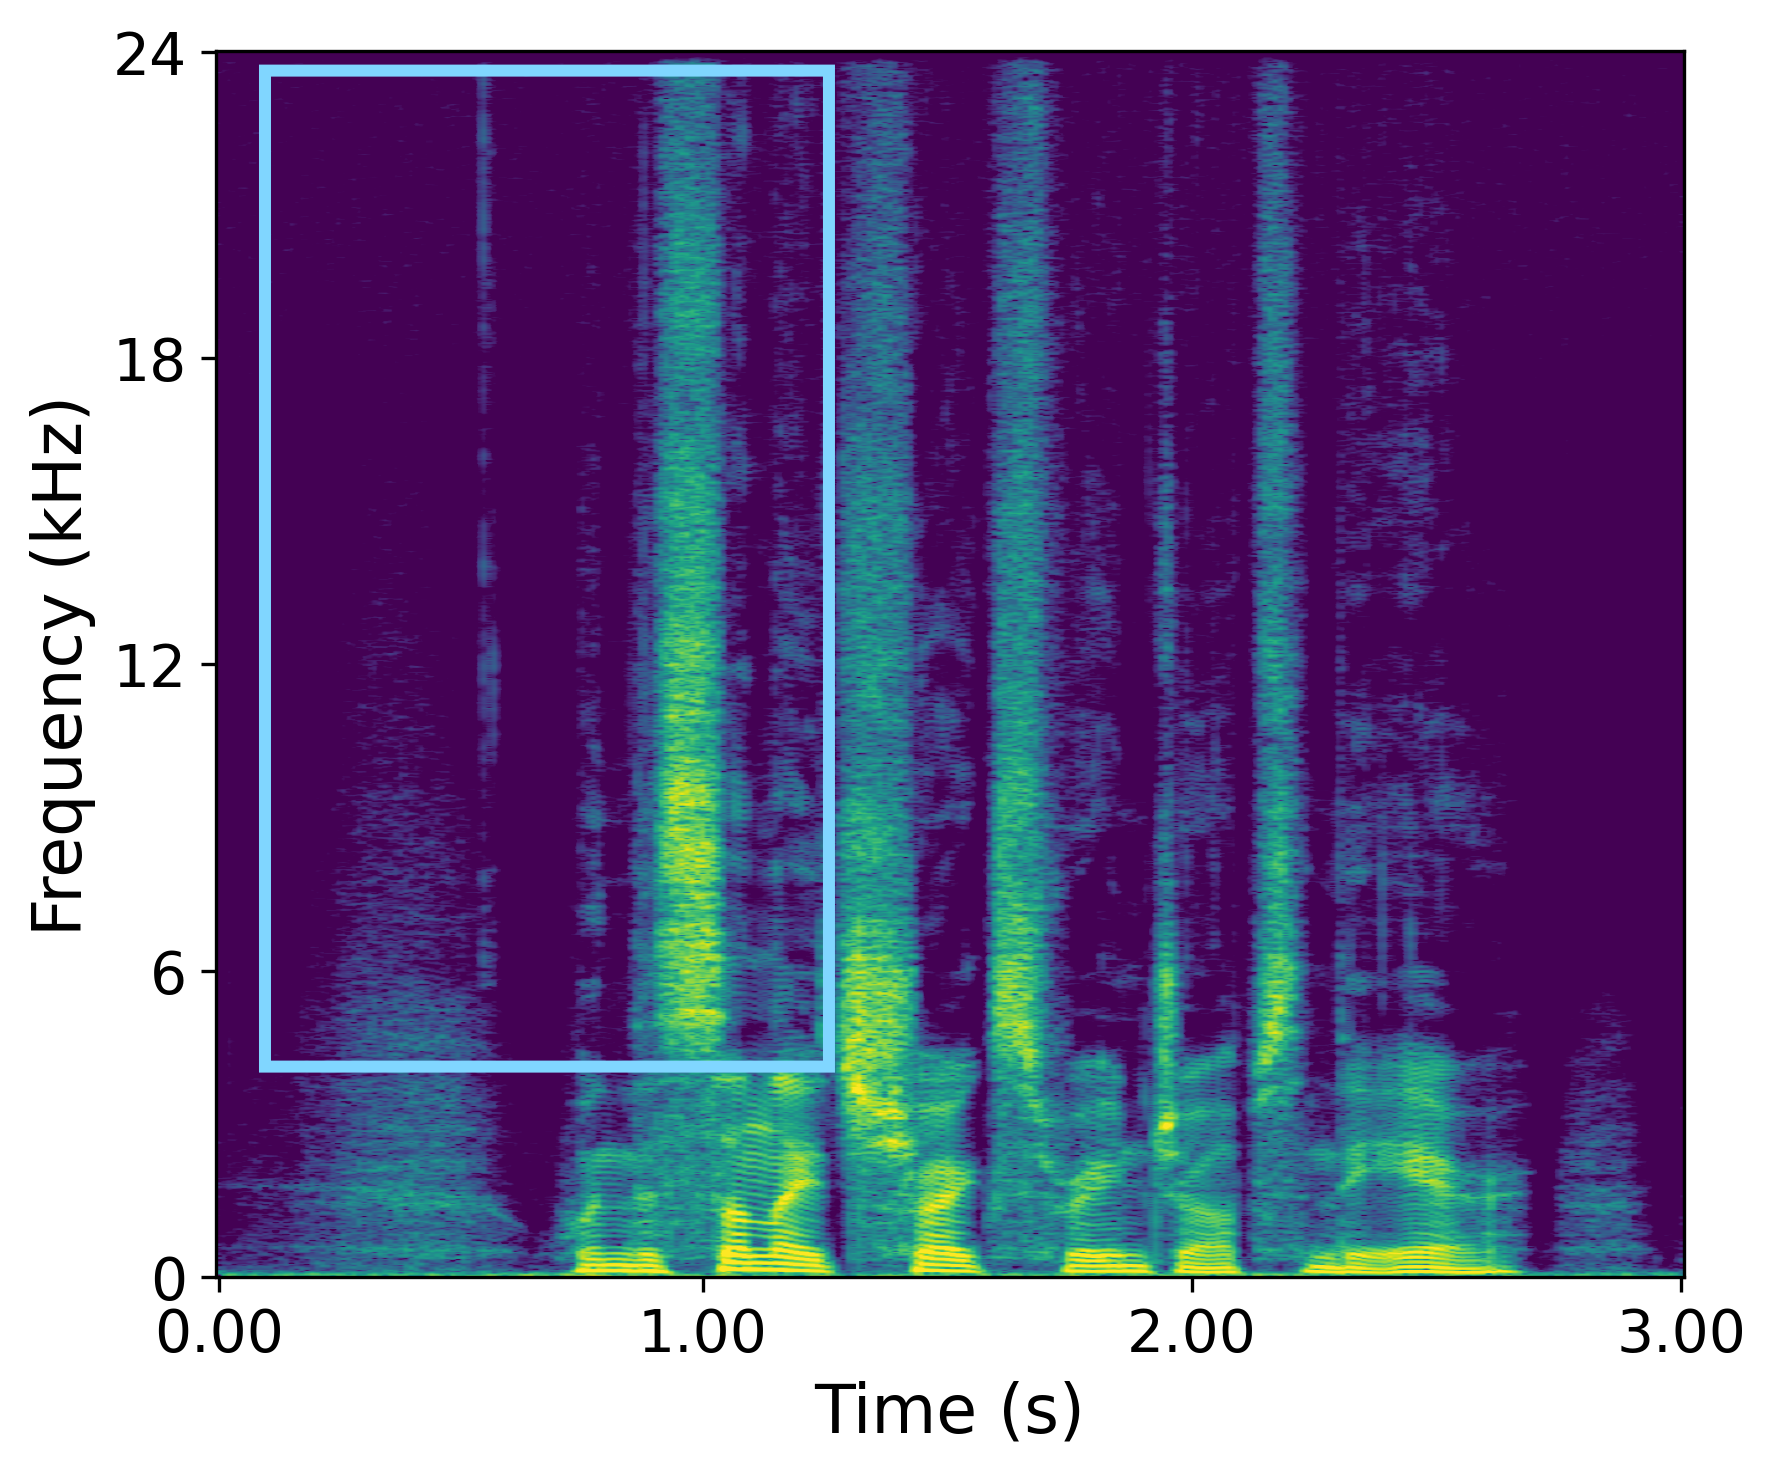
\includegraphics[width=0.48\columnwidth, trim=5 5 5 5, clip]{pic/Target.png}}
    \hfill
    \subfloat[Input $\text{LSD}=3.5918$]{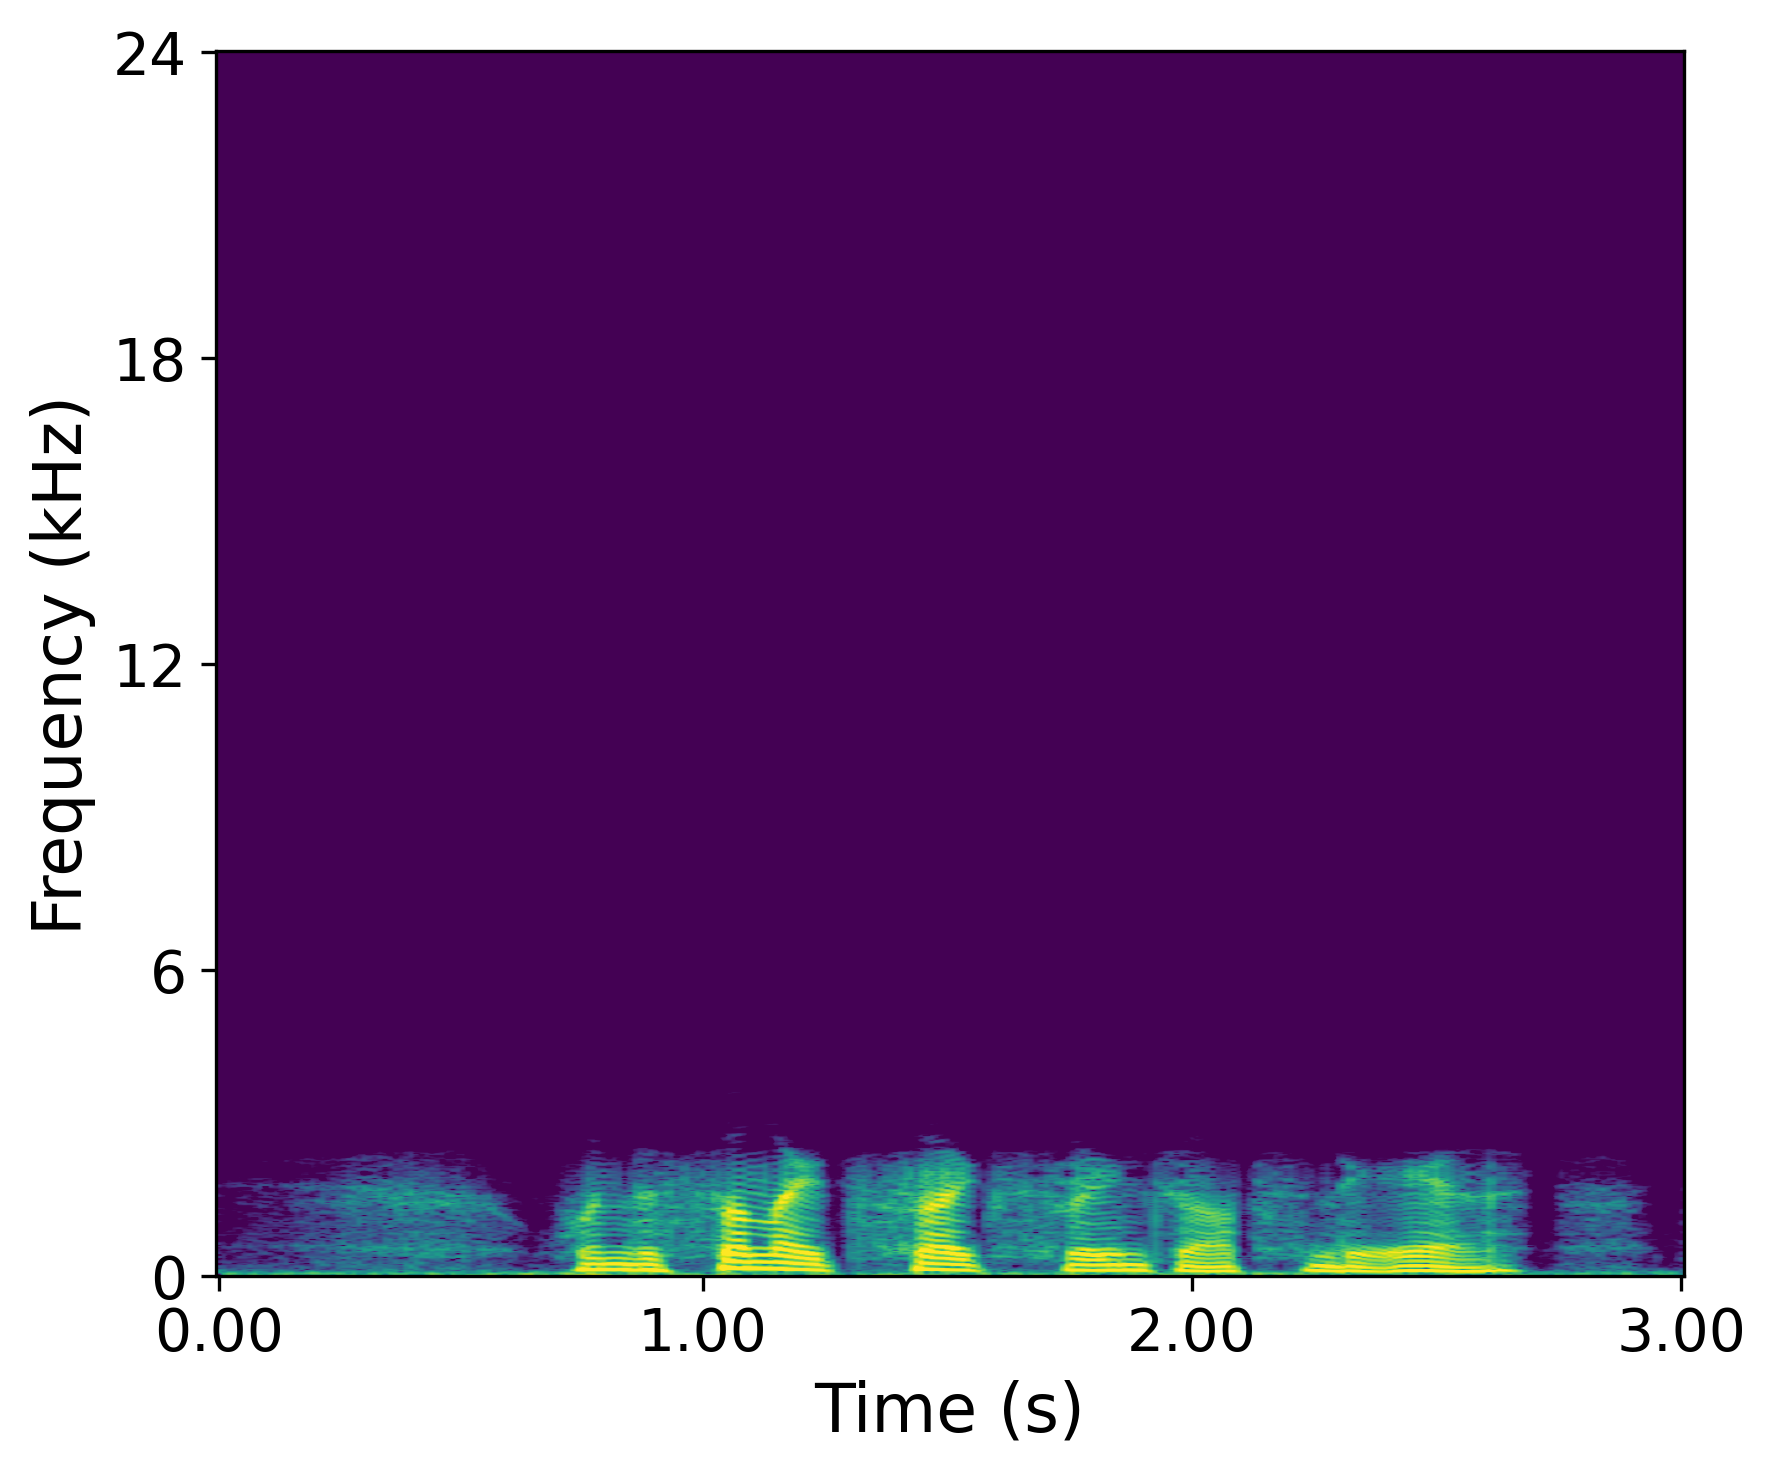
\includegraphics[width=0.48\columnwidth, trim=5 5 5 5, clip]{pic/Unprocessed.png}}
    
    \vspace{-0.3cm} 

    \subfloat[FSC-Net $\text{LSD}=0.8863$]{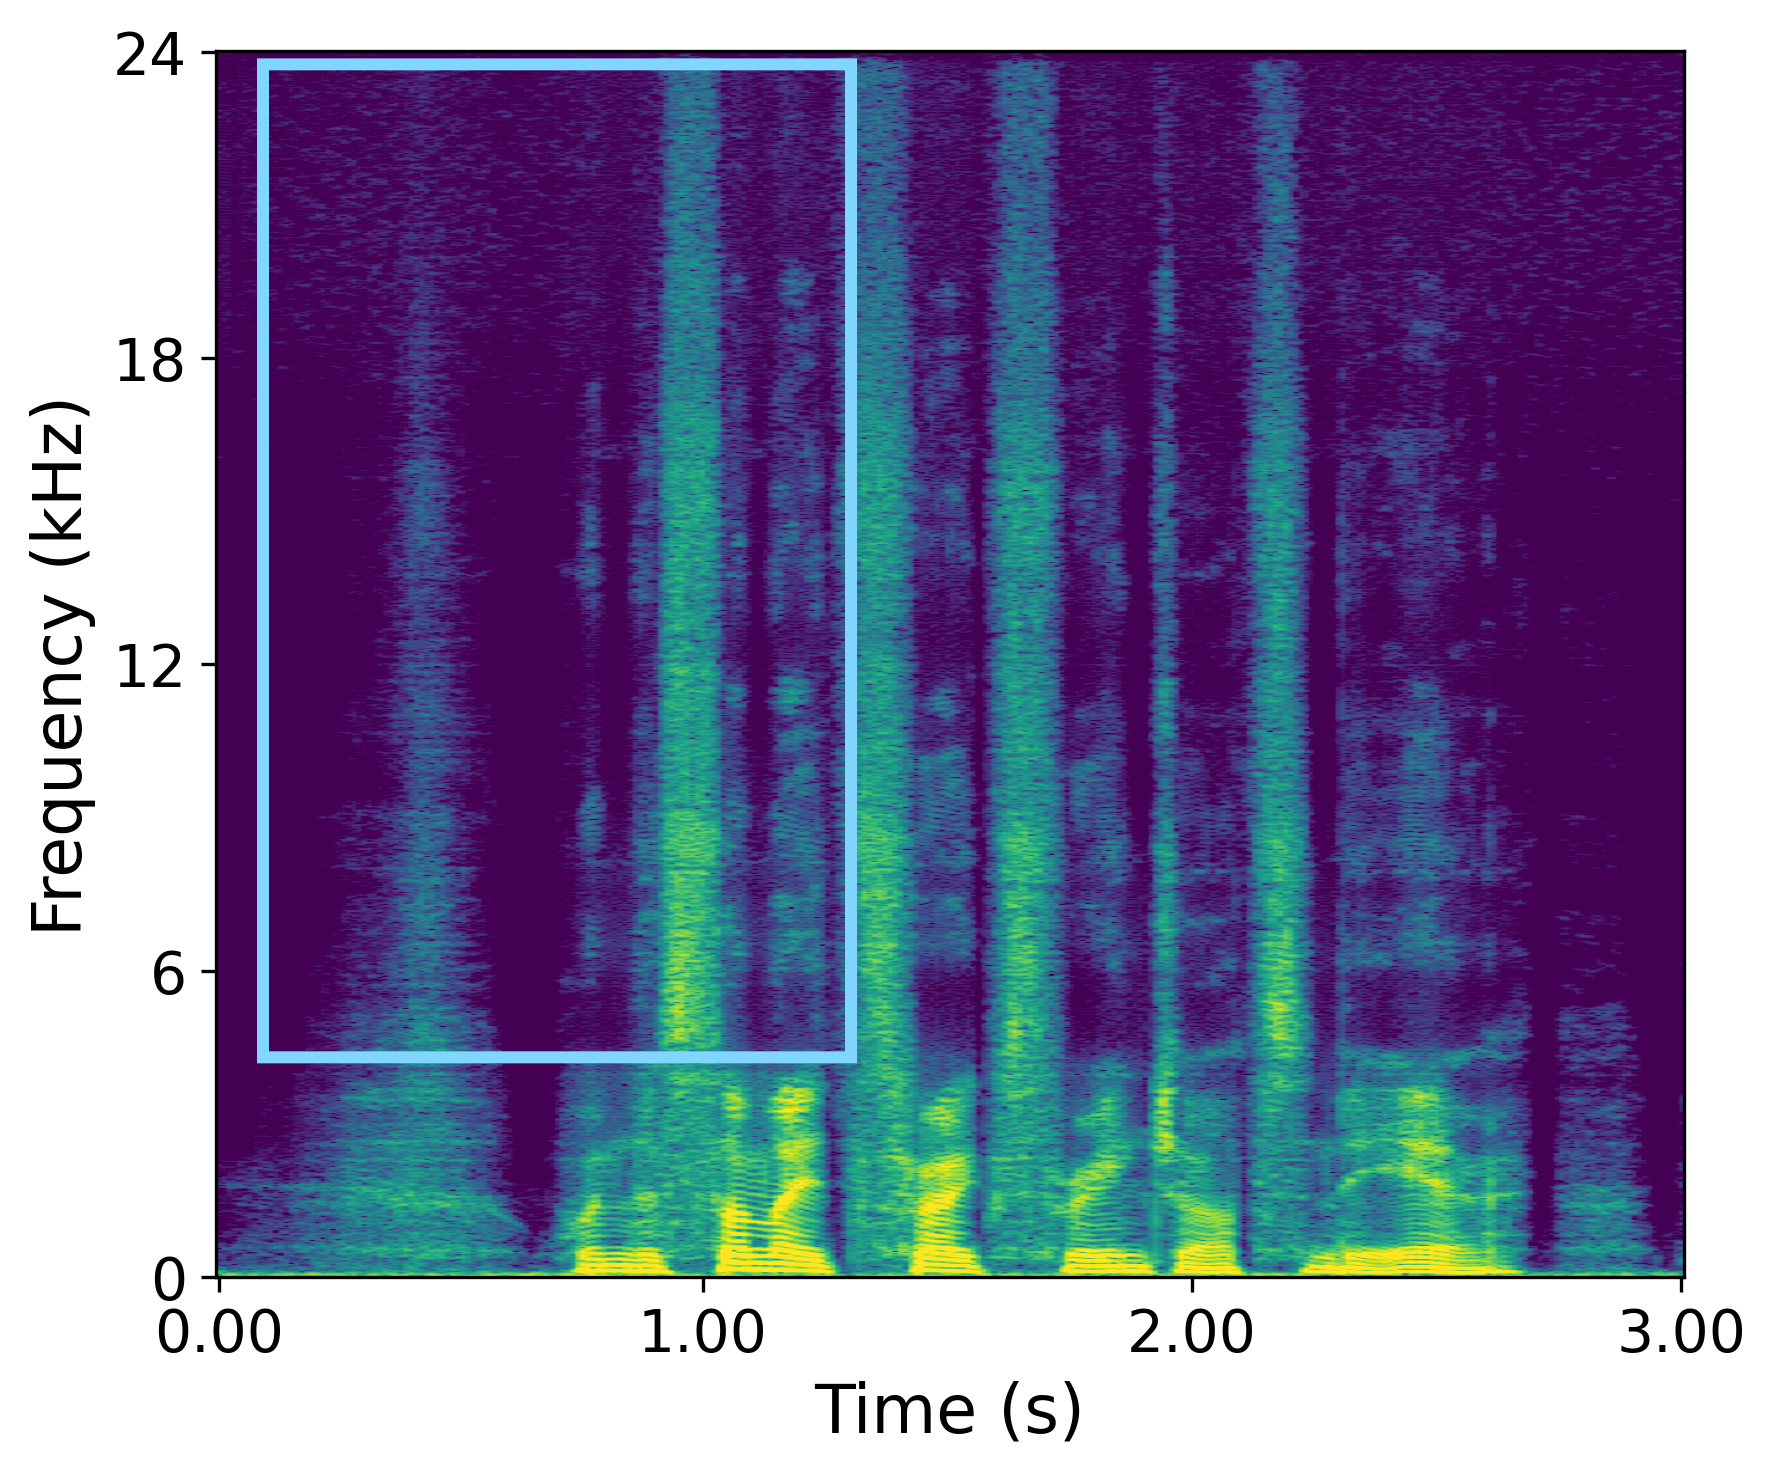
\includegraphics[width=0.48\columnwidth, trim=5 5 5 5, clip]{pic/Ours.png}}
    \hfill
    \subfloat[AP-BWE $\text{LSD}=1.0929$]{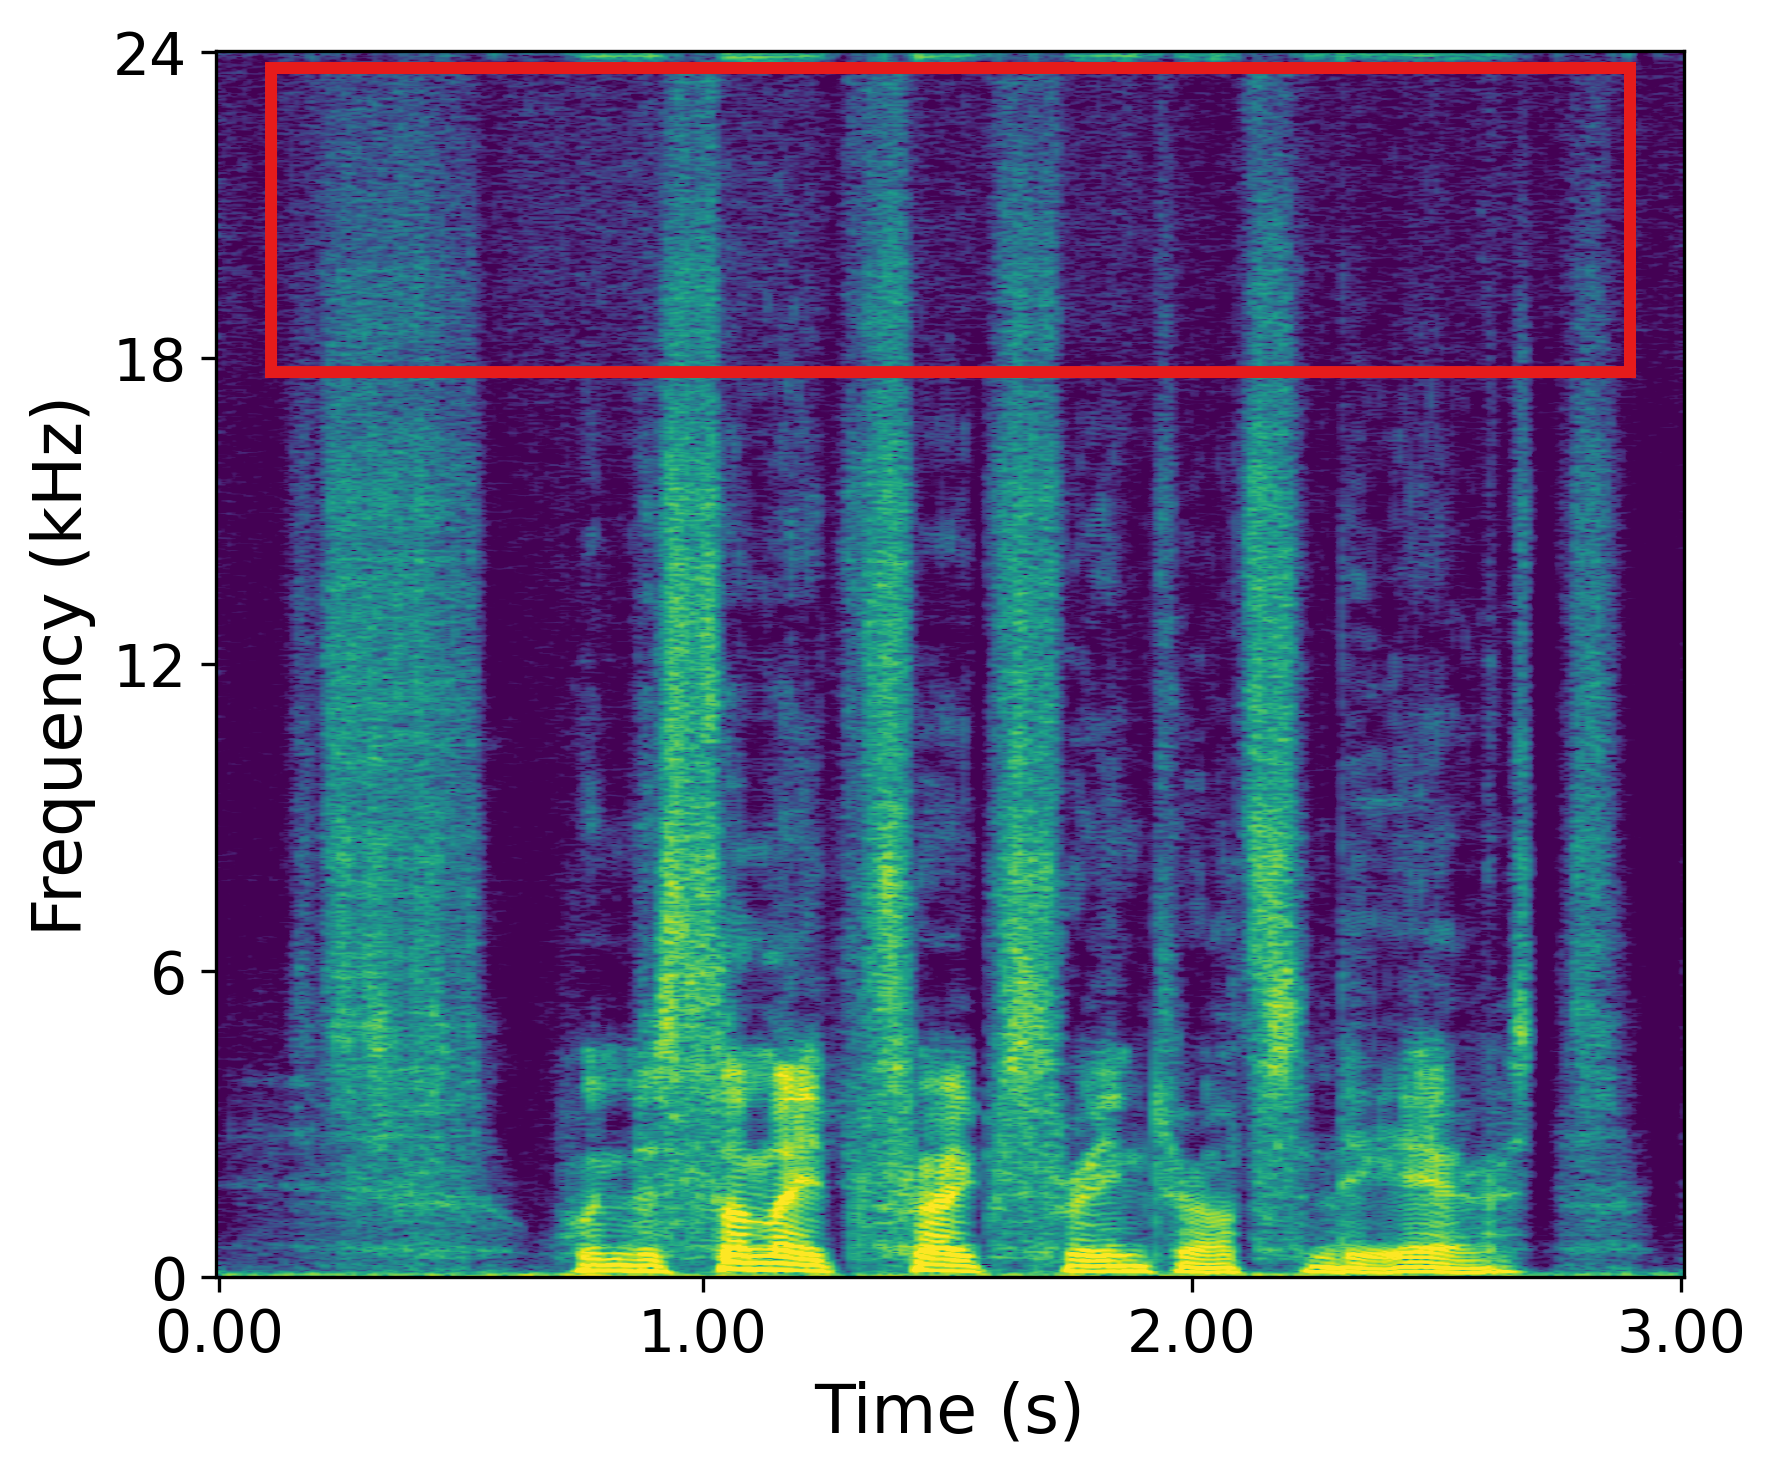
\includegraphics[width=0.48\columnwidth, trim=5 5 5 5, clip]{pic/APBWE.png}}
    
    \vspace{-0.3cm}
    
    \subfloat[BAE-Net $\text{LSD}=0.9953$]{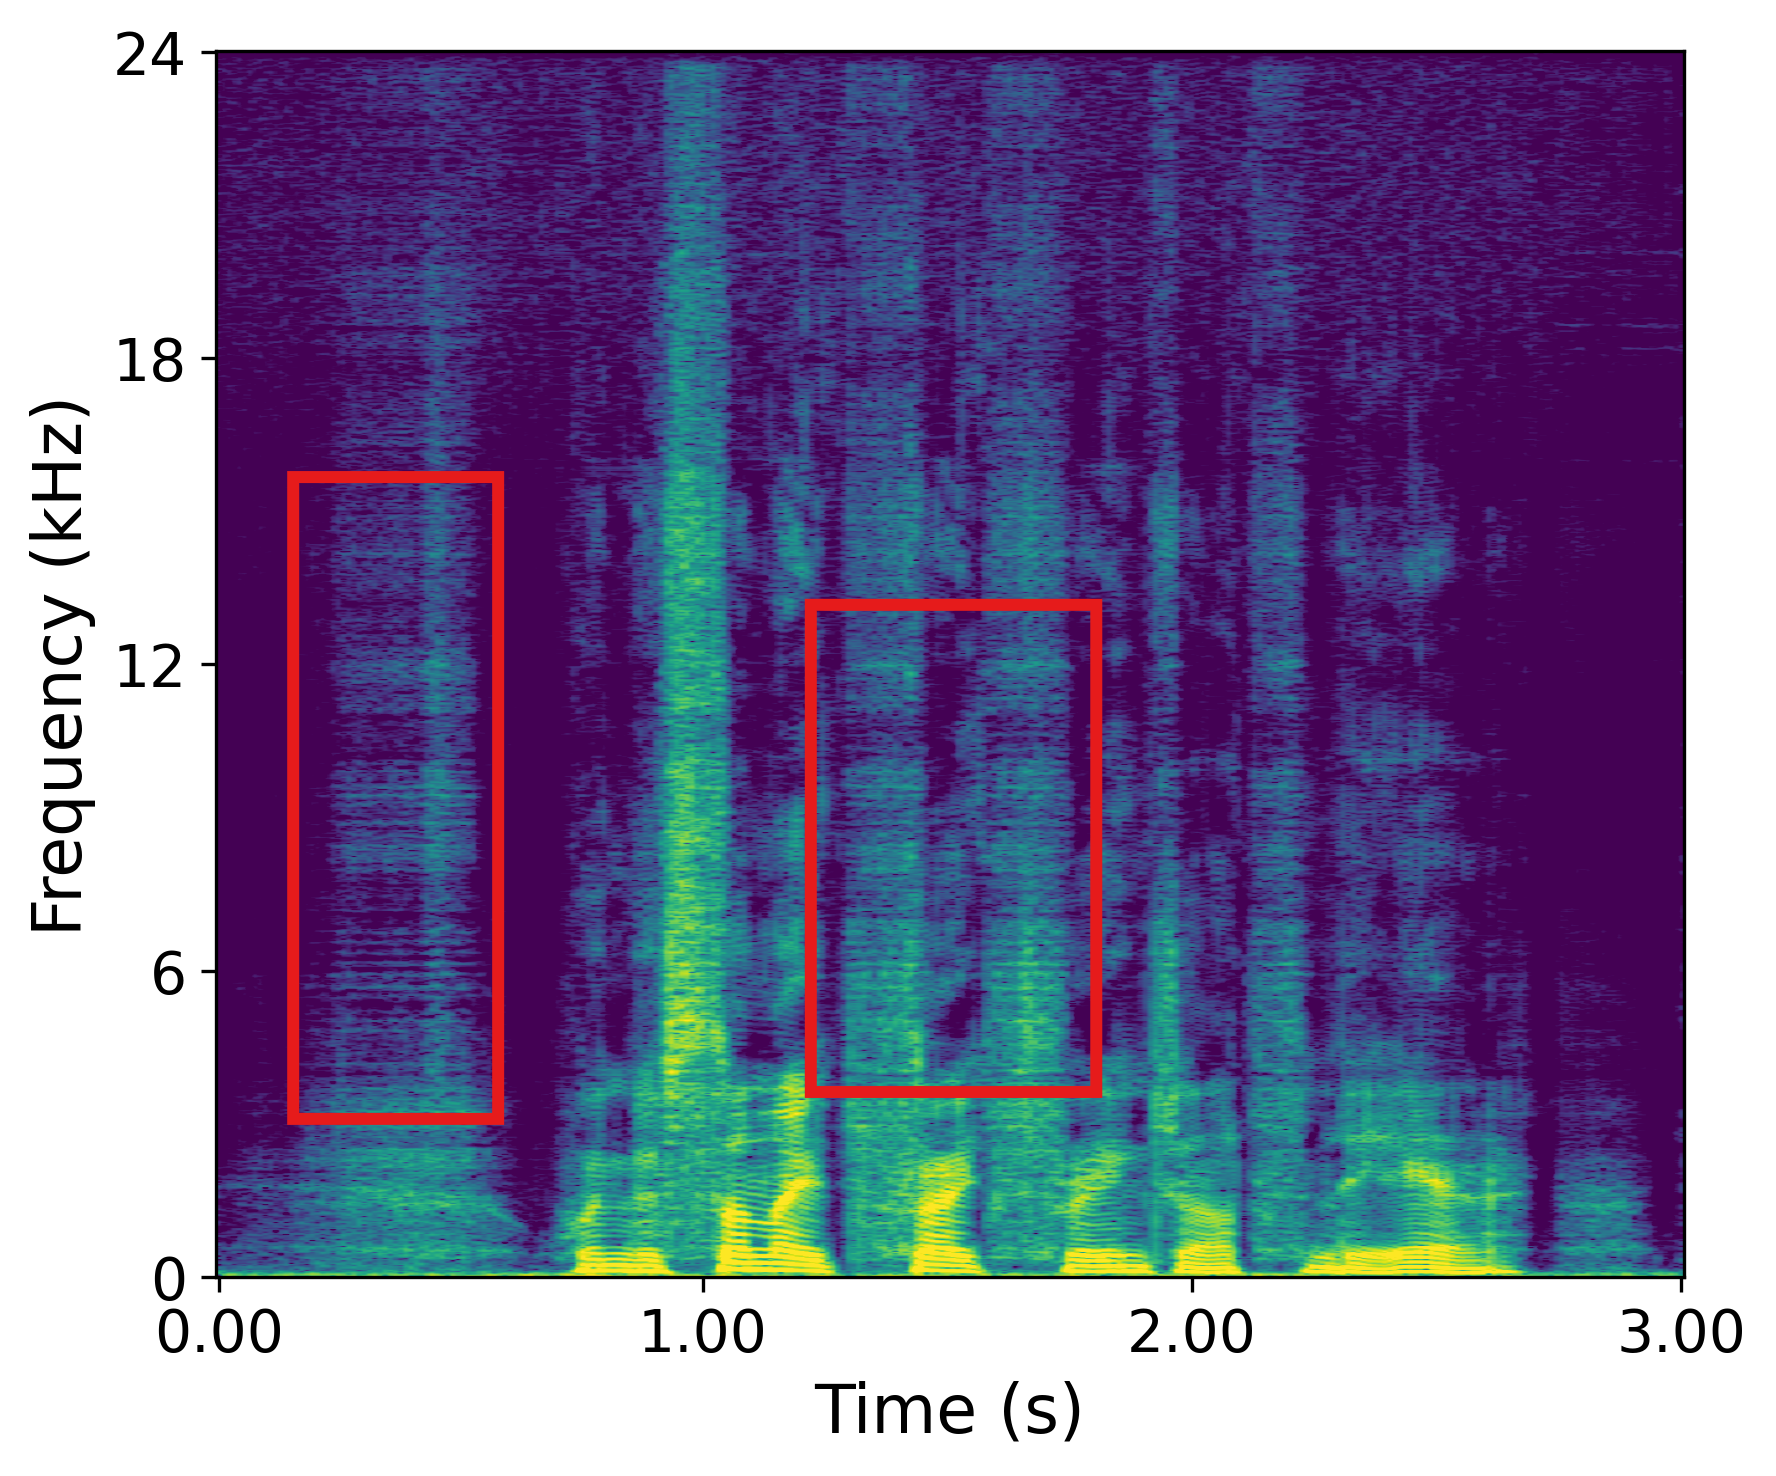
\includegraphics[width=0.48\columnwidth, trim=5 5 5 5, clip]{pic/BAENet.png}}
    \hfill
    \subfloat[AERO $\text{LSD}=0.9168$]{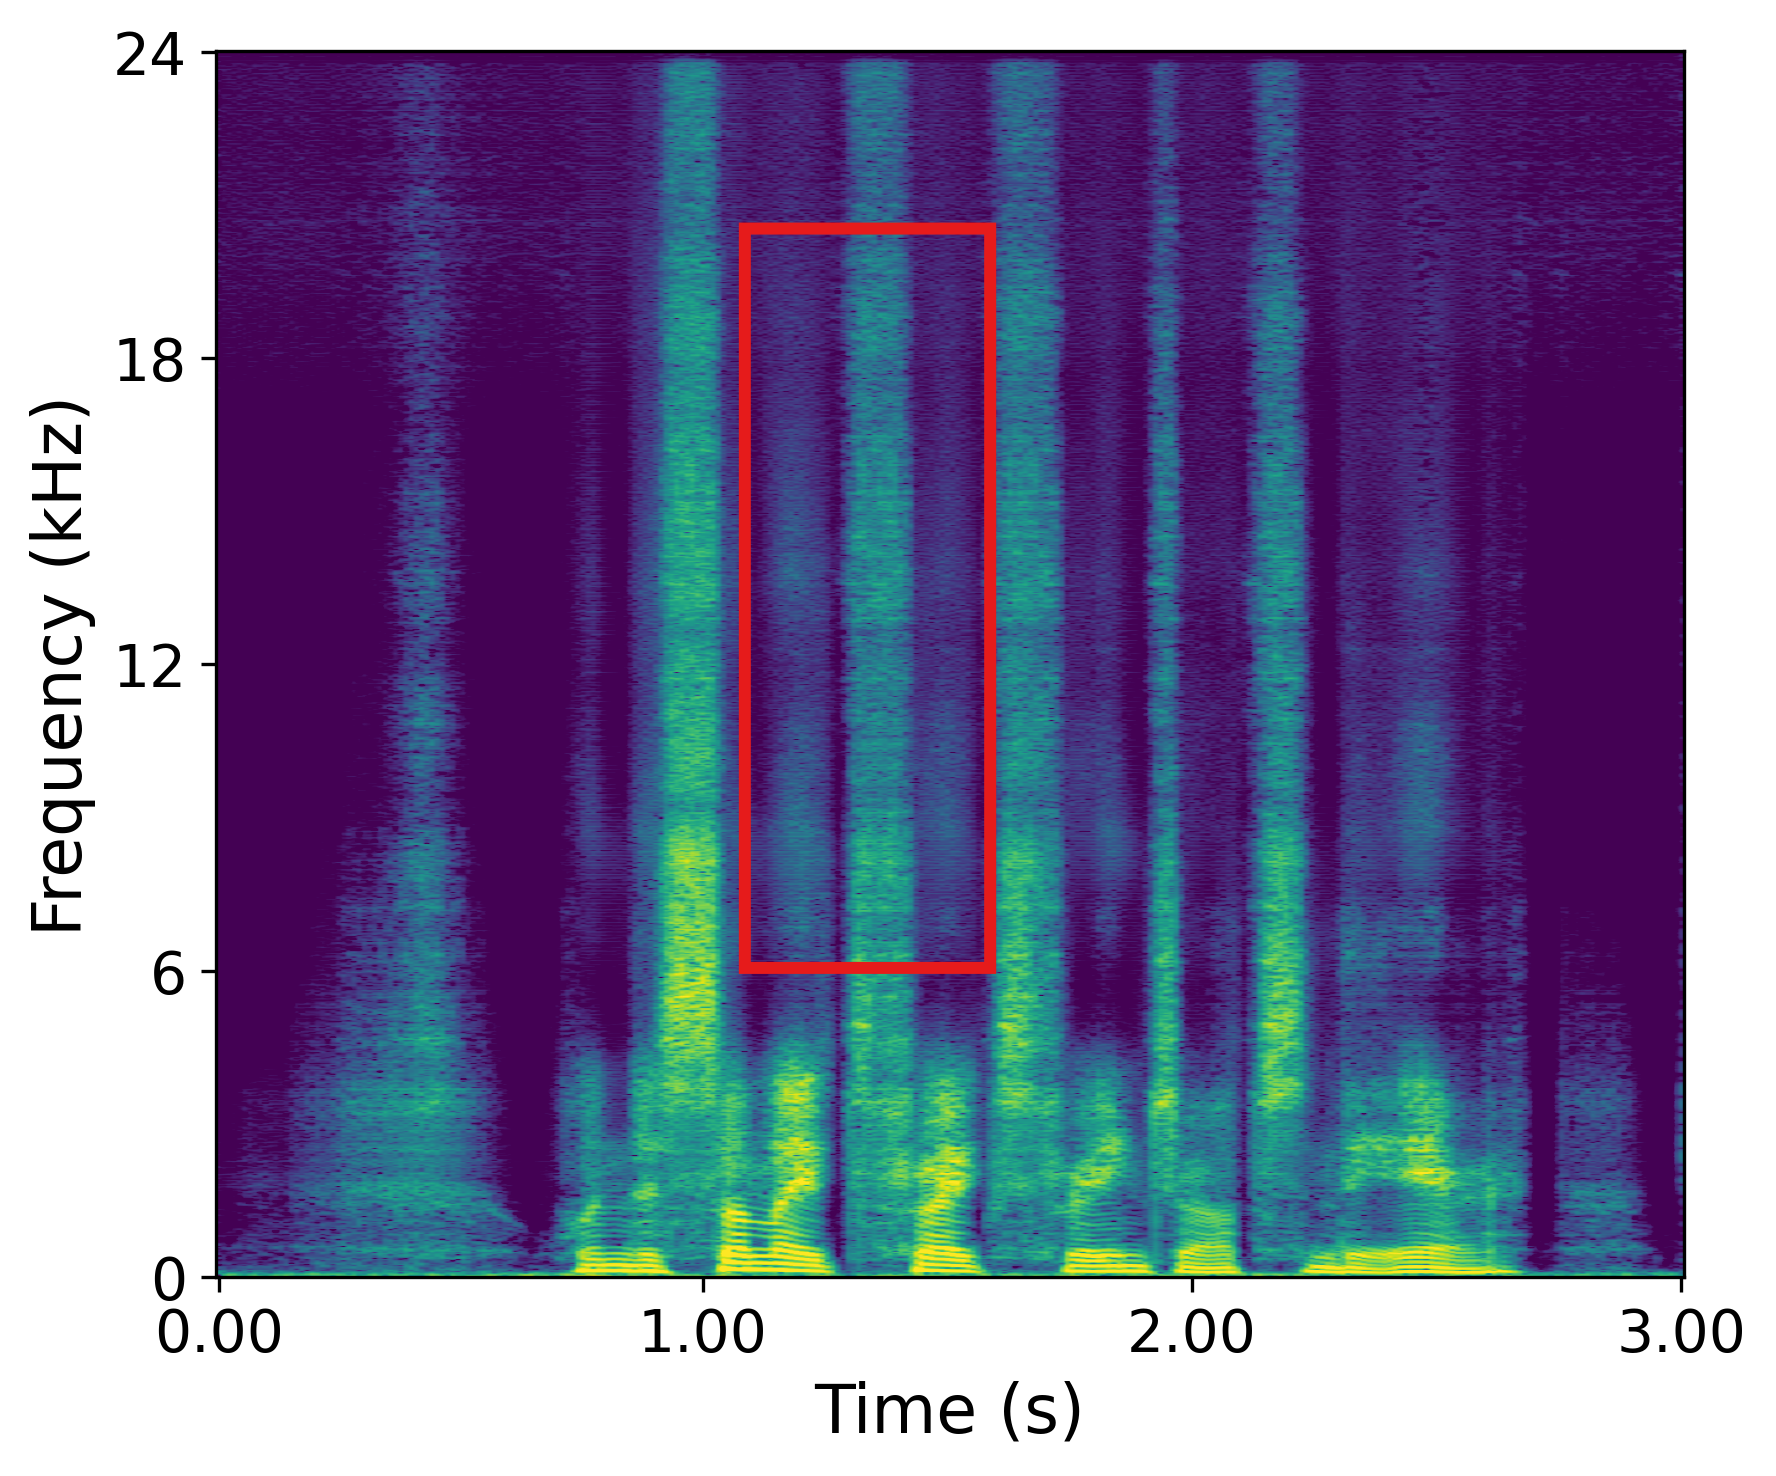
\includegraphics[width=0.48\columnwidth, trim=5 5 5 5, clip]{pic/AERO.png}}
    
    \vspace{-0.1cm}
    \caption{Spectrogram comparison of different models on the VCTK dataset (4~kHz~$\to$~48~kHz). The \textbf{blue boxes} highlight regions where our proposed FSC-Net successfully reconstructs continuous and clear high-frequency harmonic structures closely resembling the Target. Conversely, the \textbf{red boxes} indicate typical generation artifacts in baseline models: excessive high-frequency energy accumulation (AP-BWE), spectral discontinuities with insufficient energy (BAE-Net), and artificial horizontal striations with over-smoothed textures (AERO).}
    \label{fig:spec}
    
    \vspace{-0.2cm} 
\end{figure}



\subsection{Ablation Study}
We conducted an ablation study to verify the contribution of each proposed component. The results are summarized in Table \ref{tab:ablation}.
We started with the base TF-GridNet model adapted for BWE using Channel-wise Subband processing (Model A). 

\begin{table}[htbp]
\caption{Ablation Study on Proposed Components}
\label{tab:ablation}
\centering
\resizebox{\columnwidth}{!}{
\begin{tabular}{l|c|c|c}
\hline
\textbf{Model Configuration} & \textbf{LSD} $\downarrow$ & \textbf{NISQA} $\uparrow$ & \textbf{PESQ} $\uparrow$ \\
\hline
A: TF-GridNet-cws (Baseline) & 0.8843 & 4.2033 & 2.5219 \\
B: + FFC & 0.8857 & 4.2412 & 2.7011 \\
C: + FFC + Progressive Learning & \textbf{0.8771} & \textbf{4.3134} & \textbf{2.8092} \\
\hline
\end{tabular}
}
\vspace{-0.1cm}
\end{table}


\textbf{Effect of FFC:} Integrating the Fast Fourier Convolution module (Model B) improves the NISQA score from 4.20 to 4.24 and PESQ from 2.52 to 2.70 compared to the baseline. This indicates that the global receptive field provided by FFCs helps the model capture long-range spectral correlations, which are crucial for inferring missing high frequencies.

\textbf{Effect of Progressive Learning:} Introducing the frequency-progressive learning strategy (Model C) further boosts the NISQA score to 4.31 and PESQ to 2.81. Although the LSD score shows a slight improvement, the significant increase in perceptual metrics confirms that the curriculum learning approach~\cite{bengio2009curriculum}—reconstructing spectral details from coarse to fine—enables the model to generate more realistic and pleasant speech signals.

\section{Conclusion}
We proposed FSC-Net for high-fidelity speech bandwidth extension, which integrates Fast Fourier Convolutions with a frequency-progressive learning strategy to bridge the spectral gap and reconstruct realistic high-frequency content. Experiments on VCTK and the unseen EARS dataset show that FSC-Net attains leading LSD and PESQ scores against state-of-the-art baselines—including computationally scaled-up ones—while keeping a compact parameter footprint.


\bibliographystyle{IEEEtran}
\bibliography{ref.bib}

\end{document}
